\documentclass[conference]{IEEEtran}
\IEEEoverridecommandlockouts
% The preceding line is only needed to identify funding in the first footnote. If that is unneeded, please comment it out.
\usepackage{cite}
\usepackage{amsmath,amssymb,amsfonts}
\usepackage{algorithmic}
\usepackage{graphicx}
\usepackage{textcomp}
\usepackage{xcolor}
\usepackage{hyperref}
\usepackage[portuguese]{babel}
\def\BibTeX{{\rm B\kern-.05em{\sc i\kern-.025em b}\kern-.08em
    T\kern-.1667em\lower.7ex\hbox{E}\kern-.125emX}}
\begin{document}

\title{Sistema embarcado com Raspberry Pi para controle de acesso baseado em reconhecimento de placas veículares\\
{\footnotesize Projeto Final de Sistemas Operacionais Embarcados}
% \thanks{Identify applicable funding agency here. If none, delete this.}
}

\author{\IEEEauthorblockN{Gabriel Roberto Lima}
\IEEEauthorblockA{\textit{Engenharia Eletrônica - Faculdade do Gama} \\
\textit{Universidade de Brasília}\\
Brasília, Brasil \\
gabrielrobertolima@gmail.com}
\and
\IEEEauthorblockN{Matheus Alves do Nascimento}
\IEEEauthorblockA{\textit{Engenharia Eletrônica - Faculdade do Gama} \\
\textit{Universidade de Brasília}\\
Brasília, Brasil \\
alves.nascimento@aluno.unb.br}
% \and
% \IEEEauthorblockN{3\textsuperscript{rd} Given Name Surname}
% \IEEEauthorblockA{\textit{dept. name of organization (of Aff.)} \\
% \textit{name of organization (of Aff.)}\\
% City, Country \\
% email address or ORCID}
% \and
% \IEEEauthorblockN{4\textsuperscript{th} Given Name Surname}
% \IEEEauthorblockA{\textit{dept. name of organization (of Aff.)} \\
% \textit{name of organization (of Aff.)}\\
% City, Country \\
% email address or ORCID}
% \and
% \IEEEauthorblockN{5\textsuperscript{th} Given Name Surname}
% \IEEEauthorblockA{\textit{dept. name of organization (of Aff.)} \\
% \textit{name of organization (of Aff.)}\\
% City, Country \\
% email address or ORCID}
% \and
% \IEEEauthorblockN{6\textsuperscript{th} Given Name Surname}
% \IEEEauthorblockA{\textit{dept. name of organization (of Aff.)} \\
% \textit{name of organization (of Aff.)}\\
% City, Country \\
% email address or ORCID}
}

\maketitle

\begin{abstract}

\end{abstract}

\begin{IEEEkeywords}

\end{IEEEkeywords}

\section{Introdução}
Atualmente, a adoção das tecnologias de automação residencial se tornou amplamente difundida, especialmente em grandes condomínios, oferecendo inúmeros benefícios em termos de conforto e segurança para os residentes. Uma prática comum é a abertura dos portões por meio de dispositivos de controle remoto que utilizam radiofrequência. No entanto, esse método de acionamento requer que o usuário sempre tenha o controle em suas mãos e ainda demanda certo tempo no manuseio do dispositivo representando, em alguns casos, um risco para a segurança do usuário.

Visando a solução desses problemas, a proposta consiste na implementação de um sistema embarcado de reconhecimento de placas veiculares para controle de acesso utilizando \textit{Raspberry Pi} aliado à tecnologias de processamento de imagens como a biblioteca openALPR que apresenta soluções de Automatic License Plate Recognition - ALPR, utilizada por BUHUS et al.\cite{b1}. Outros trabalhos, como ABIRAMI et al.\cite{b2} e ULLAH et al. \cite{b3} também obtêm bons resultados de reconhecimento com o uso da biblioteca OpenCV, da qual o OpenALPR deriva.

Tomando como base os trabalhos apresentados anteriormente, pretende-se realizar o reconhecimento da existência do veículo e posteriormente a identificação do mesmo através da placa. Caso a placa esteja cadastrada como acesso permitido o portão é aberto, caso contrário o portão permanecerá fechado. 

Para a melhor experiência com o usuário, com o auxílio da plataforma de mensagens \textit{telegram}, é possível cadastrar as placas referentes aos veículos e saber quando acessam as dependências do condomínio.

Atualmente algumas empresas oferecem o mesmo tipo de serviço, como a \href{https://www.secticom.com.br/lpr-controle-de-acesso-por-leitura-de-placa/}{Secticon} na qual oferece serviços de monitoramento e vigilância no Brasil inteiro. Encontramos ainda câmeras de reconhecimento como a câmera feita pela  \href{https://www.intelbras.com/pt-br/camera-ip-com-leitura-automatica-de-placas-vip-7250-lpr-ia-ft-g2}{IntelBrás} e \href{https://www.hikvision.com/pt-br/newsroom/blog/managing-vehicle-entry-with-anpr/}{Hikivision}. Essas duas empresas oferecem soluções muito próximas ao proposto pelo projeto para o mercado. As câmeras fabricada, tanto pela IntelBrás quanto pela Hikivision, apresentam diversas funções. Além do reconhecimento das placas, realiza identificação de cor e marca dos veículos, e exporta relatórios de acesso dos veículos capturados. Apresenta integração com outros dispositivos como alarmes e botoeiras através de conexões próprias com outros dispositivos das fabricantes, sendo inclusive utilizadas em sistemas de automação de estacionamentos. 

O sistema a ser desenvolvido deve ser capaz de capturar imagens, realizar o acionamento de um controle e a leitura de sensores ultrassônicos para iniciar o processo de reconhecimento de veículos. Além disso, deve ser feito o reconhecimento das placas das imagens capturadas e realizar comunicação com o \textit{Telegram}.

\section{Desenvolvimento}
\subsection{Descrição de Hardware}

\subsubsection{\textit{Bill of Materials - BOM}}

\begin{itemize}
    \item Raspberry Pi 4
    \item Fonte 5V 3A
    \item Cartão SD
    \item Câmera (\textit{webcam})
    \item Controle Remoto 433 MHz (Modificado)
    \item Transistor NPN - BD139
    \item 6 resistores 1k$\Omega$
    \item 2 sensores ultrassônicos HC-SR04

\end{itemize}


\subsubsection{Diagrama de Blocos}

\begin{figure}[!h]
    \centering
    \includegraphics[width = \linewidth]{Imagens/Diag_SOE.png}
    \caption{Diagrama de blocos do projeto}
    \label{fig:diagBlocos}
\end{figure}

O projeto é composto por um diagrama de blocos \ref{fig:diagBlocos} simples, com a Raspberry Pi ocupando o papel central, onde todas as informações são processadas. A partir dela, temos diversos módulos interligados, incluindo uma fonte de alimentação que fornece energia para todo o sistema, uma câmera encarregada de capturar imagens para o reconhecimento de placas de veículos, sensores ultrassônicos para identificar a presença de veículos, um controle modificado que a Raspberry Pi opera e, posteriormente, aciona o portão, e também a comunicação com o aplicativo de mensagens \textit{Telegram}, que possibilita a verificação de veículos autorizados, o cadastro de novos veículos e a execução de outros comandos essenciais no sistema.\\

\subsubsection{Esquemático}

O diagrama esquemático foi projetado dividindo as partes e integrando posteriormente. À esquerda um circuito com os sensores ultrassônicos foi implementado, atentando-se para a tensão de sinal enviada pelo sensor, que deve ser adequada por meio de um divisor resistivo com resistores de $1k\Omega$ e $2k\Omega$, fornecendo tensão de saída de aproximadamente $3.3V$, afim de não danificar as portas GPIO da Raspberry Pi, haja vista que a tensão de saída do sinal dos sensores é de $5V$.

O controle foi modificado de forma que ao fornecer tensão para o mesmo, ele é acionado, ignorando seu botão. O fornecimento tensão (5V) na base do transistor, ativa o controle. 

Por fim, a Raspberry Pi, recebe ligação da fonte de alimentação e câmera utilizada para captação de imagens no projeto. 

\begin{figure}[h]
    \centering
    \includegraphics[width=0.9\linewidth]{Imagens/Esquemático.png}
    \caption{Esquemático do projeto}
    \label{fig:esquema}
\end{figure}


\subsection{Descrição de software}
\subsubsection{Fluxograma}

O sistema de monitoramento de entrada de veículos segue as etapas apresentadas na figura \ref{fig:fluxograma}. Tudo começa quando um veículo se aproxima da área de entrada e é detectado pelos dois sensores ultrassônicos seguindo a máquina de estados da figura\ref{fig:maqEstados}. Uma vez que o veículo é detectado, o sistema captura uma imagem do veículo, incluindo a placa, usando uma câmera. Essa etapa é essencial para a identificação do veículo.
O sistema utiliza elementos de \textit{Machine Learning} para detecção de veículo. Caso a acuse a presença de um carro, o sistema aciona o um algoritmo que reconhece caracteres e faz a leitura da placa. Com esses dados, o sistema prossegue com a consulta a um banco de dados de autorizações. Neste banco de dados, são armazenados os padrões de números e letras autorizados a entrar no edifício ou condomínio.

\begin{figure}
    \centering
    \includegraphics[width=0.7\linewidth]{Imagens/maq_estados.png}
    \caption{Máquina de estados para acionamento do sistema}
    \label{fig:maqEstados}
\end{figure}

O sistema verifica se a combinação de números e letras lida na placa do veículo está autorizada no banco de dados. Se a combinação for encontrada no banco de dados, o veículo é considerado autorizado.

Caso o veículo seja autorizado, o sistema envia um sinal para o controle remoto do portão, permitindo a abertura do portão de entrada desejado. Após a entrada bem-sucedida do veículo autorizado, o sistema envia uma notificação, via Telegram, para informar que um veículo específico entrou no local. Isso é útil para manter um registro de entrada e saída.

Além disso, o sistema permite que novas placas sejam cadastradas no banco de dados via Telegram. Os usuários podem enviar as informações da placa juntamente com a autorização via Telegram, e o sistema atualizará o banco de dados com as informações da placa autorizada. Com a conclusão do processo, o sistema volta ao estado de espera, pronto para detectar o próximo veículo que se aproxima da área de entrada.


\begin{figure}[h]
    \centering
    \includegraphics[width=0.7\linewidth]{Imagens/Fluxograma.png}
    \caption{Fluxograma do Projeto}
    \label{fig:fluxograma}
\end{figure}

O software é projetado para monitorar a entrada de veículos em um edifício ou condomínio. Utiliza uma série de bibliotecas para realizar as tarefas necessárias:


\begin{itemize}
\item \textbf{wiringPi:} Controla os pinos GPIO da Raspberry Pi para dispositivos de detecção, como sensores ultrassônicos, e atua no controle do portão
\item \textbf{Stdlib:} Realiza operações de alocação de memória e conversão de tipos de dados.
\item \textbf{Stdio:} Facilita a comunicação com o usuário, a leitura e escrita de informações, como configurações e logs do sistema.
\item \textbf{Pthread:} Permite a execução simultânea de tarefas, como detecção de veículos e notificações.
\item \textbf{String:} É usada para manipular e validar as placas dos veículos, bem como para a comparação com os dados do banco de dados de autorização.
\item \textbf{Unistd:} Arquivo de cabeçalho que fornece acesso à API do POSIX.
\item \textbf{Telebot:} Interage com a API do Telegram, permitindo que o sistema envie notificações e comunique-se com os administradores.
\item \textbf{OpenCV:} Processa e analisa imagens para a leitura das placas dos veículos, incluindo detecção de bordas, segmentação de caracteres e reconhecimento óptico de caracteres (OCR).
\item \textbf{Tesseract:} Realiza a detecção de caracteres alfanuméricos com auxílio da biblioteca OpenCV
\item \textbf{Yolo:} Faz a detecção de objetos através de \textit{Machine Learning}.

Em conjunto, essas bibliotecas habilitam o sistema a detectar veículos, ler suas placas, consultar autorizações no banco de dados, controlar o portão, enviar notificações via Telegram e analisar as placas. O software oferece um sistema eficiente e completo para o monitoramento de entrada de veículos.

O software foi desenvolvido para atuar com dois processos simultâneas. Um primeiro processo rodará o \textit{bot telegram} e o outro fará a captura da foto, a análise da placa e acionamento do portão. Esses processos se comunicam através de arquivos que armazenam dados de placas e identificadores do telegram.

O \textit{loop} principal do processo do \textit{bot} aguarda o envio de mensagem de algum usuário. Assim que a mensagem é recebida, o mesmo verifica se o usuário inseriu algum dos comandos pré-definidos para registro e exclusão de placas e inclusão no recebimento de notificações. Caso nenhuma dessas funções seja acionada, a mensagem retornada apresenta os comandos disponíveis para o usuário. Todos os comandos realizam alterações em arquivos. 

O comando "/Adicionar" realiza a escrita da placa informada pelo usuário no arquivo "placas.lp", cada placa em uma linha. 

A função "/Remover" fará a gravação de todas as placas já registradas, exceto a placa informada pelo usuário, em um arquivo temporário. Em seguida, o programa exclui o arquivo de placas e renomeia o arquivo temporário com o nome do arquivo de placas para uso posterior. 

O comando "/Notificacao" permite o usuário escolher se deseja ou não receber notificações através do aplicativo \textit{Telegram}. Para isso, o "id" do usuário é adicionado à um arquivo, "notificados.nf", que será utilizado posteriormente para envio das notificações de entrada pelo portão. 

O processo responsável pela verificação das placas inicia verificando o estado de cada um dos sensores ultrassônicos. À medida que eles são acionados em uma ordem pré-estabelecida \ref{fig:maqEstados}, o sistema desencadeia outros processos. Quando detecta-se a presença de um veículo, a câmera é acionada e tira uma foto da placa do veículo. A imagem é processada pela ferramenta \textit{Yolo} que identifica se há ou não um carro. Em seguida, é realizado o reconhecimento de caracteres. O texto obtido é comparado com os números de placa gravados no arquivo mencionado anteriormente. Caso a placa reconhecida estiver no arquivo, a entrada é liberada realizando o acionamento do controle por "GPIO". Neste mesmo momento, todos os telefones inclusos no arquivo de notificados, receberão uma notificação de acesso ao portão pela placa. 

\section{Resultados}

\subsection{Acionamento Controle}

Para ativar o controle, um algoritmo em C controla a porta \textit{GPIO} com auxilio da biblioteca \textit{WiringPi}. Ao ser executado, a porta GPIO 18 é habilitada com tensão 5V durante 1 segundo e em desliga. 

\subsection{Sensores Ultrassônicos}

Um sinal é enviado para os pinos de \textit{trigger} dos sensores ultrassônicos pelo pino 16, e os sinais recebidos como retorno do sensor são lidos pelos pinos 18 e 22. O algoritmo calcula o tempo de retorno do sinal enviado e retorna uma distância em centímetros e apresenta no terminal. Além do estado da máquina de estado da figura \ref{fig:maqEstados}. O arranjo e o resultado obtido são apresentados nas figura \ref{fig:teste_us1} e \ref{fig:teste_us2}.

\begin{figure}[h]
    \centering
    \includegraphics[width=0.8\linewidth]{Imagens/teste_ultrassom.png}
    \caption{Teste sensor ultrassônico}
    \label{fig:teste_us1}
\end{figure}

\begin{figure}[h]
    \centering
    \includegraphics[width=0.8\linewidth]{Imagens/teste_ultrassom_lab.png}
    \caption{Teste sensor ultrassônico - Bancada}
    \label{fig:teste_us2}
\end{figure}


\subsection{Comunicação Telegram}

Para testes com o Telegram, foi utilizada a biblioteca Telebot com um \textit{echobot} fornecido pela própria biblioteca. Um \textit{bot} foi criado com auxilio do \textit{botFather}. O exemplo utilizado apresenta um texto recebido e reenvia novamente para o usuário no aplicativo de mensagens. O código rodando na Raspberry Pi esta rodando o recebimento de dados na figura \ref{fig:telegram_test}

\begin{figure}[h]
    \centering
    \includegraphics[width=0.8\linewidth]{Imagens/telegram.png}
    \caption{Teste de \textit{bot Telegram}}
    \label{fig:telegram_test}
\end{figure}

\subsection{Câmera}

Para captura das imagens com a câmera, foi utilizado um algoritmo pronto em C que utiliza comandos da biblioteca \textit{opencv}. Abaixo um exemplo de imagem capturada com a câmera \ref{fig:cam}. 

\begin{figure}[h]
    \centering
    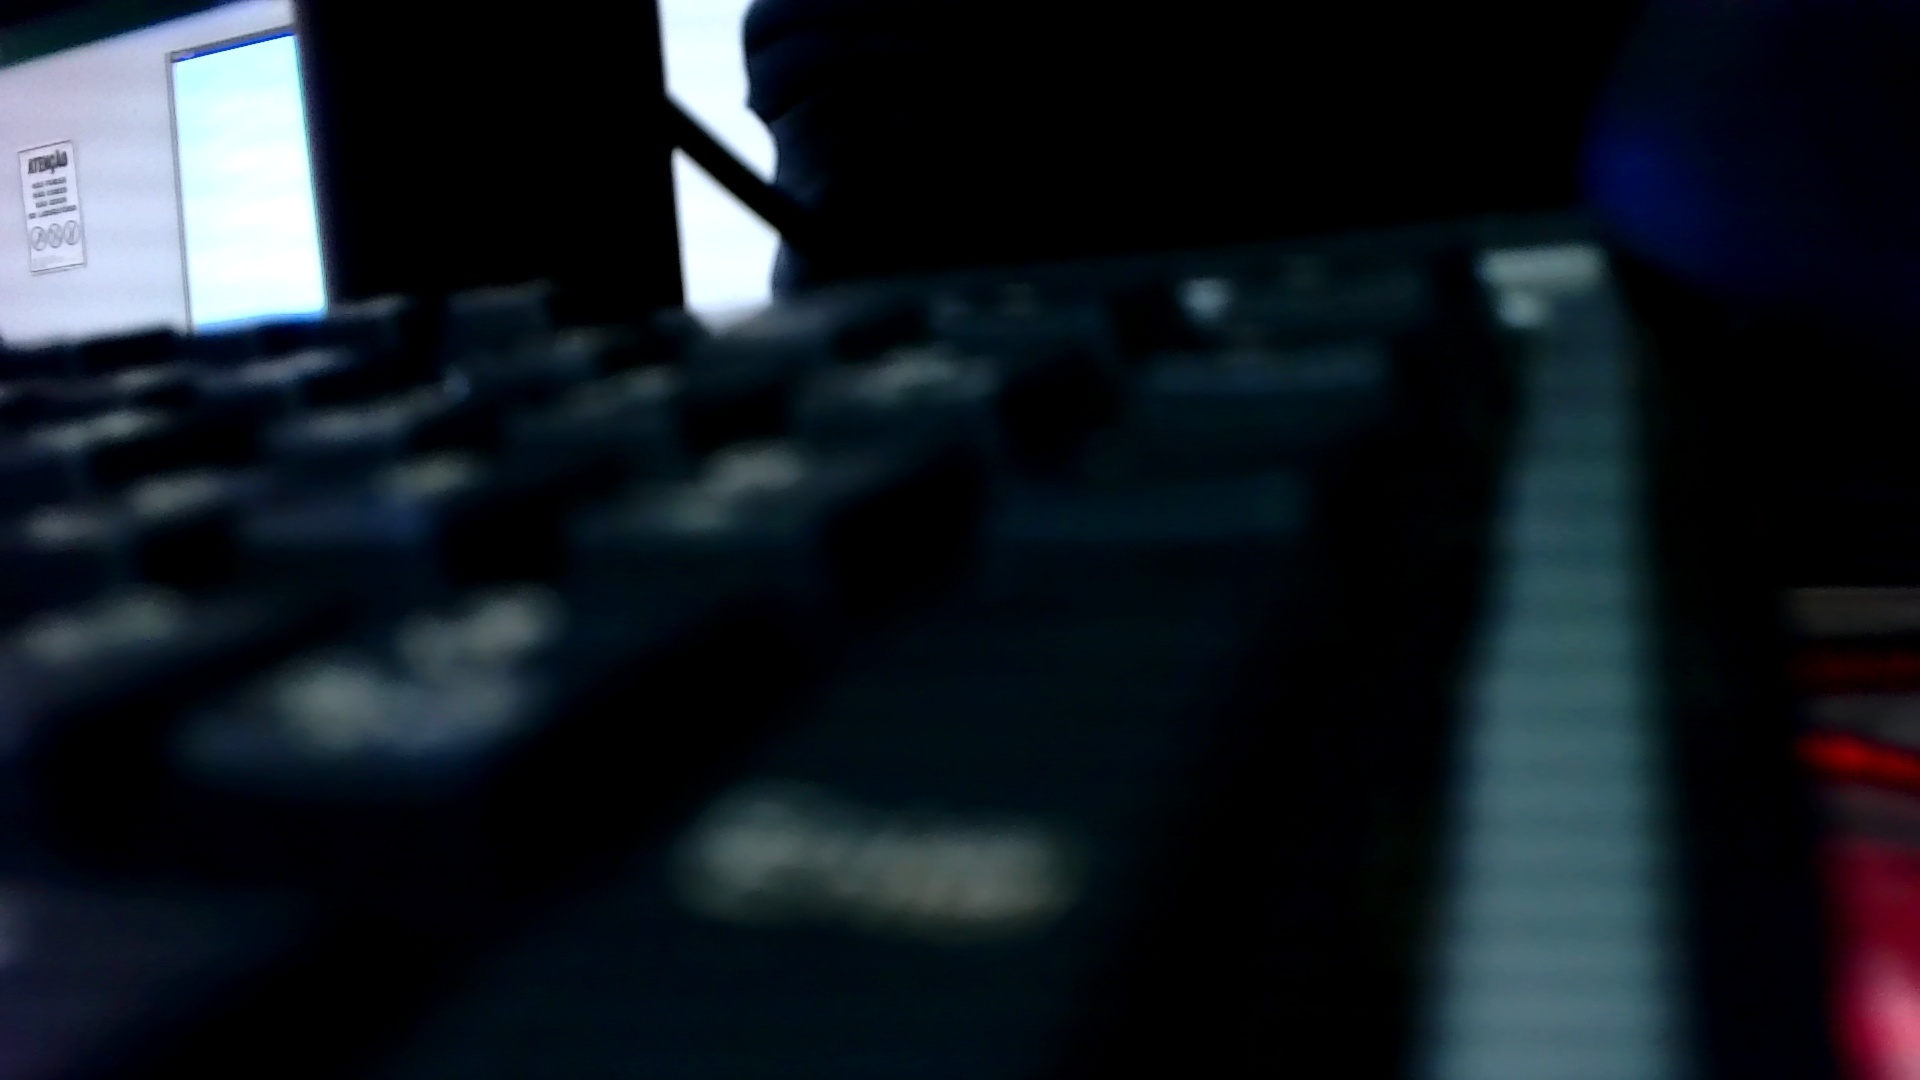
\includegraphics[width=0.8\linewidth]{Imagens/captured_image.jpg}
    \caption{Imagem capturada com a \textit{webcam}}
    \label{fig:cam}
\end{figure}

\subsection{Reconhecimento de veículos e caracteres de placas}

Para o reconhecimento de carros, é utilizada a ferramenta Yolo, e a imagem \ref{fig:carro}, que retorna o reconhecimento de um carro, conforme \ref{fig:respYolo}.

\begin{figure}[h]
    \centering
    \includegraphics[width=0.7\linewidth]{Imagens/retorno_yolo.png}
    \caption{Resposta Yolo com a imagem de um carro}
    \label{fig:respYolo}
\end{figure}

\begin{figure}[h]
    \centering
    \includegraphics[width=0.7\linewidth]{Imagens/carro.jpg}
    \caption{Imagem de carro feita com a própria WebCam do projeto}
    \label{fig:carro}
\end{figure}

O reconhecimento dos caracteres das placas é feito pela biblioteca \textit{Tesseract}. E, utilizando a mesma imagem \ref{fig:carro}, retorna o resultado apresentado na imagem \ref{fig:respTesseract}.

\begin{figure}
    \centering
    \includegraphics[width=0.7\linewidth]{Imagens/retorno_tesseract.png}
    \caption{Retorno de algoritmo com a biblioteca Tesseract}
    \label{fig:respTesseract}
\end{figure}
\newpage
\begin{thebibliography}{00}
\bibitem{b1} BUHUS, Elena Roxana; TIMIS, Daniel; APATEAN, Anca. Automatic parking access using openalpr on raspberry pi3. Acta Technica Napocensis, v. 57, n. 3, p. 10, 2016.

\bibitem{b2} ABIRAMI, N.; JASMINE, JS Leena. Accurate vehicle number plate recognition and real-time identification using raspberry pi. International Research Journal of Engineering and Technology (IRJET), v. 5, n. 04, p. 7, 2018.

\bibitem{b3} ULLAH, Farman et al. Barrier access control using sensors platform and vehicle license plate characters recognition. Sensors, v. 19, n. 13, p. 3015, 2019.

\bibitem{b4} LPR – Reconhecimento de placas de veículos-https://www.secticom.com.br/lpr-controle-de-acesso-por-leitura-de-placa/

\bibitem{b5}Câmera IP com leitura automática de placas- https://www.intelbras.com/pt-br/camera-ip-com-leitura-automatica-de-placas-vip-7250-lpr-ia-ft-g2

\bibitem{b5}https://www.hikvision.com/pt-br/newsroom/blog/managing-vehicle-entry-with-anpr/

https://www.hikvision.com/pt-br/newsroom/blog/managing-vehicle-entry-with-anpr/



\end{thebibliography}

\end{document}
